\chapter{Grundlagen}

Zunächst wird auf den Aufbau und Features von Bildern eingegangen. Zur Detektion und Extraktion von Features aus Bildern haben sich zahlreiche verschiedene Verfahren etabliert. Von diesen wird der SIFT Feature Detektor und Deskriptor näher betrachtet, da er im Weiteren als Basis für die Feature Gewinnung dient. Es werden anschließend Modelle vorgestellt, die sich mit der Reduzierung der Dimensionen der Features beschäftigt, um eine Repräsentation zu erhalten, dich sich effizient vergleichen lässt. Das Bag of Visual Words Modell wurde aus dem Bereich Information Retrival adaptiert und wir zur Klassifizierung von Bildern auf Basis lokaler Features verwendet. Alternativ zu diesem Ansatz wird der Autoencoder vorgestellt. Ein Autoencoder ist ein spezielles neuronales Netzwerk, dass selbständig eine komprimierte Darstellung der Eingabe, in diesem Fall die Bild Features, lernt. Im letzten Teil wird auf die Berechnung allgemein mathematischer Probleme auf Grafikkarten, das GPGPU Programming eingegangen. Durch den Einsatz von Grafikkarten können Berechnungen gerade bei großen Datenmengen stark beschleunigt werden, da diese massiv parallel auf den Daten arbeiten. Mit Nvidias cuda wird eine Sprache vorgestellt mit der sich Modelle wie Bag of Words und Autoencoder auf Nvidia Hardware realisieren lassen.

\section{Bilder und Features}

Ein Bild kann mathematisch als eine Funktion $I$ aufgefasst werden, die jeden Punkt an der Position $(x, y)$ des Bildes auf seinen Farb- bzw. Intensitätswert abbildet. Ein Punkt ist je nach Darstellung unterschiedlich repräsentiert. Bei einem Graustufenbild handelt es sich um einen Intensitätswert zwischen 1 und 256. Bei Darstellung in Farbe besteht der Punkt aus roten, grünen und blauen Anteilen mit einem Wert zwischen 1 und 256. Bei dem Vergleich von Bildern werden diese Punkte, ihre Eigenschaften und u. a. ihr Nachbarschaft betrachtet. Globale Verfahren berücksichtigen bei der Bewertung jeden Punkt des Bildes gleichermaßen, lokale hingegen betrachten nur ein kleines Fenster des Bildes, dafür meist mehrere. Die Suche nach globalen Merkmalen, im Weiteren auch Features genannt, die ein Bild charakterisieren kann aber keine Objekte und Details im Bild berücksichtigen. Hierfür eignet sich die Extraktion von lokalen Features. Um Objekte aus unterschiedlichen Perspektiven und in verschiedenen Größen wieder zu erkennen, ist es notwendig, dass die Features affin invariant sind. Folgende Abbildung zeigt dasselbe Objekt, jedoch rotiert, skaliert und verschoben. Ein Algorithmus sollte mit hoher Wahrscheinlichkeit erkennen, dass es sich hier um dasselbe Objekt handelt.

Warum Features? -> Nicht nur Position / Bedeckung, generelle Eigenschaften (anhängig vom Deskriptor)

BEISPIEL BILD

Die Gewinnung der Features ist in zwei Schritte aufgeteilt: Zuerst ermittelt ein Detektor Muster, die sogenannten \textit{interest points}. Muster können anhängig vom Detektor Punkte, Linien oder Regionen sein. Durch das lokale Vergleichen von Punkten und deren Nachbarschaft werden diese effizient ermittelt. Bei der Wahl des Detektors sollte die angestrebte Allgemeinheit berücksichtigt werden: Ein Feature Detektor für medizinische Bilder spezieller Annahmen treffen, als einer für eine allgemeine Bildsuche. Anschließend wird durch die Feature Extraktion aus den \textit{intereset points} der Deskriptor erzeugt, eine kompakte Darstellung des Features für die weitere Verarbeitung. 

SIFT ist ein von Lowe entwickeltes Verfahren zur Feature Extraktion und Detektion. Bei der Detektion von Features werden Rotationen, Skalierungen und Translationen von gefundenen Features erkannt und diese durch Den Deskriptor als ein Histogramm der Orientierungen dargestellt. Im Folgenden wird die Funktionsweise von Histogrammen vorgestellt und dann das SIFT Verfahren erläutert.

\cite{ifd2016}

\subsection{Histogramme}

Ein Histogramm ist eine diskrete Funktion, welche die Häufigkeitsverteilung einer Menge abbildet. Hierfür wird jeder Wert der Menge einer Klasse zugeordnet. Jede Klasse umfasst einen vorher definierten Wertbereich. Im Bereich der Bildverarbeitung wird beispielsweise oft die Verteilung der Punkte auf die Intensitäten betrachtet. Im Falle eines Graustufenbildes liegen 256 Klassen vor. Beim bilden des Histogramms wird jeder Punkt betrachtet und der Zähler der Klasse um eins inkrementiert, in deren Wertebreich der Intensitätswert des Punktes fällt. Ein Histogramm ist normalisiert, wenn die Anzahl der Werte einer Klasse durch die Anzahl der Gesamtwerte dividiert wird.
In Abbildung \ref{img:hist} sind im Wesentlichen zwei Bereiche zu erkennen: ein sehr hellerer Hintergrund und eine dunkle Katze, die den Großteil des Bildes ausmacht. Dies spiegelt sich auch im Histogramm wieder: Es ist eine große Mengen an Punkten im dunklen Bereich vorhanden (Intensität < 128) und eine kleine, extreme Häufung im hellen Bereich.

\begin{figure}
	\centering
	\includegraphics[scale=0.8]{images/big_cat.png}
	\caption{Graustufenbild und Verteilung der Intensitätswerte}
	\label{img:hist}
\end{figure}

\subsection{Scale-invariant feature transform}

SIFT ist ein Feature Detektor und Deskriptor der 1999 von Lowe entwickelt wurde. Die von SIFT entdeckten Features sind (affin?) invariant und beschreiben die Nachbarschaft des keypoints. Der Algorithmus ist in vier Schritte unterteilt:

\begin{enumerate}
	\item \textbf{Detektion von Extremen im Maßstab} Die \textit{keypoints} werden durch einen Difference of Gaussians (DOG) Filter ermittelt. Das Bild wird durch eine Konvolution mit einem gausschen Kernel $G(x, y, d)$ geglättet, wobei $d$ die Standardabweichung ist. Dadurch das nur räumliche Informationen höherer Bereiche unterdrückt werden, fungiert dies als Band Pass Filter und hebt so die Sichtbarkeit von Kanten hervor. Der Lapalacien of Gaussian wird dann durch die Differenz zweier Gaussians berechnet. Dabei ist die Standardabweichung des Minuenden $k$ mal größer, als die des Subtrahenden. In der Praxis hat sich beim Einsatz in SIFT der Wert $k = 1.4$ bewährt. Die Extrempunkte aus einer Reihe von DOG Abbildungen sind dann die Punkte, die ein lokales Minimum oder Maximum besitzen.
	\item \textbf{Keypoint Lokalisierung} Nicht alle Kandidaten werden zu \textit{keypoints}. Jeder Kandidaten muss einer Reihe von Stabilitätsmaßen genügen. Befindet sich ein Punkt auf einer Kante oder besitzt einen zu geringen Kontrast, wird er aussortiert. Dies wird durch eine Taylor Expansion zweiter Ordnung mit Ursprung im \textit{keypoint} durchgeführt.
	\item \textbf{Bestimmung der Orientierung} Bei dem Aufbau des Feature Vektoren pro \textit{interest point} wird die lokale Orientierung abgeschätzt. Auf diese Weise sind die SIFT Deskriptoren invariant gegenüber Rotationen. Der SIFT Algorithmus berechnet ein Histogramm der Orientierung der Gradienten. Hierfür werden zufällig Punkte aus der Nachbarschaft ausgewählt. Der Extremwert des Histogramms wird hier als dominante Orientierung verwendet.
	\item \textbf{Deskriptor} Für jeden durch den Detektor gefundenen keypoint wird nun ein Featurevektor gebildet. Der Featurevektor enthält Informationen über die Nachbarschaft in Form der Gradienten eines jeden Punktes in der Nachbarschaft. Das Fenster für die Auswahl der Nachbarschaft wird auf dem keypoint zentriert und in vier Teilfenster unterteilt. Die Gradienten in allen Teilfenster werden in acht Richtungen quantisiert, sodass der resultierende Deskriptor 128 Dimensionen enthält.
\end{enumerate}

\begin{figure}
	\centering
	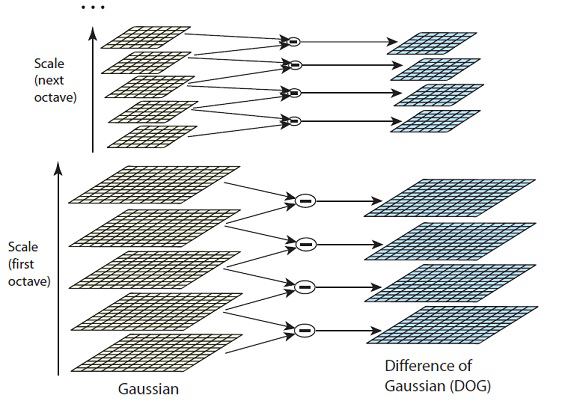
\includegraphics[scale=0.7]{images/dog.png}
	\caption{Difference of Gaussians Operator, Abbildung aus \cite{dif2004}}
	\label{img:sift_dog}
\end{figure}

PRO

\begin{enumerate}
	\item Änderungen im Grenzwert von Position und Orientierung verändern den Feature Vektor kaum.
	\item Erreicht eine kompakte Darstellung. Robustheit ist in praktischen Anwendungen enorm hoch, auch wenn der Algorithmus keine affine Invarianz bietet.
	\item In Vergleichen wurden sehr gute Ergebnisse gegen andere Algorithmen erzielt.
\end{enumerate}

CON

\begin{enumerate}
	\item Die Konstruktion des SIFT Deskriptors ist aufwendig
	\item Hohe Dimensionalität des Feature Vektors, was zu einer langen Berechnungszeit führt.
\end{enumerate}

\section{Bag of Visual Words}

Das Bag of Words Modell stammt aus dem Bereich Information Retrival und wird zur Klassifizierung von Dokumenten genutzt. Es wird das Auftreten jedes Wortes in eine Dokument gezählt und durch die Anzahl aller Wörter im Vokabular geteilt, um so einen normalisierten Wert zu erhalten.

Dieses Modell wurde von der Computer Vision adaptiert um Bilder zu klassifizieren. Die Features können aber nicht direkt statt der Worthäufigkeit verwendent werden: Ein Feature ist ein kleiner, lokaler Ausschnitt aus einem Bild und wird selten in der gleichen Form wieder auftreten. Weiterhin findet ein Detektor wie SIFT oder SUSAN ca. 100 bis 1000 Features pro Bild, daher ist es notwendig die Features zu gruppieren. Da alle Features eines Detektors die gleiche Dimension haben, können Clustering Verfahren angewendet werden um dies zu erreichen. Ein Cluster entspricht dann einem Visual Word und ist Teil des Codebooks. Durch Algorithmen wie k-means kann die Größe des Codebooks kontrolliert werden. Wurde ein Codebook aus einer Menge von Bildern erstellt, lassen sich nun weitere Bilder klassifizieren. Hierfür werden wieder die lokalen Features des Bildes extrahiert und nun alle durch ein nearest-neighbour Verfahren dem nächsten Cluster bzw. Visual Word zugewiesen und anschließend ihre relative Häufigkeit bewertet werden.

\subsection{K-Means Clustering}

Der k-means Clustering Algorithmus fasst eine Menge von Vektor gleicher Dimensionalität in eine Menge von k vorgegeben Gruppen zusammen. Auf diese Weise können Zusammenhänge in Daten entdeckt werden und auch Klassifizierungen effizient durchgeführt werden, da die Distanz eines Vektors zu jedem Cluster betrachtet werden kann und ein Maß für die Ähnlichkeit abgeleitet werden kann. Der Algorithmus geht in zwei Stufen vor:

\begin{enumerate}
	\item \textbf{Cluster bilden}: Zunächst müssen die initialen k Cluster gebildet werden. Häufig verwendete Methoden sind zufällige Auswahl und Auswahl des Vektors mit der größten Distanz zu den bisher gewählten Clustern.
	\item \textbf{Vektoren zuweisen}: Nach Auswahl der Cluster wird die Distanz eines jeden verbleibenden Vektors zu Zentrum eines jeden Cluster gemessen. Der Vektor des Paares mit der geringsten Distanz wird dem entsprechenden Cluster zugewiesen. Dieser Schritt wird solange wiederholt bis jeder Vektor einem Cluster zugewiesen wurde.
\end{enumerate}

Im Folgenden Beispiel werden statt Vektoren Punkte im zweidimensionalen Raum betrachtet. Dieser Prozess läuft für höhere Dimensionen unter Berücksichtigung der Distanzmetriken analog ab. Als k wird hier drei gewählt. Der Erste Cluster muss zufällig gewählt werden, da keine Informationen vorliegen, auf Basis derer eine gute Entscheidung getroffen werden kann. Als erstes wird der Punkt 4 gewählt. Im nächsten Schritt bestimmen wir den Punkt der am weitesten von Punkt 4 entfernt ist. Berechnet man die Distanz für alle Punkte, so sind Punkt 5 und 10 beide am weitesten und gleich weit von Punkt 4 entfernt. In diesem Fall wird zufällig Punkt 10 gewählt. Da nach ein Cluster gefunden werden muss wird nun die Distanz von jedem verbleibendem Punkt zu Punkt 4 und 10 bestimmt. Dieser Schritt liefert Punkt 1 als initialen Mittelpunkt für den dritten Cluster. \cite{mmd2011}

\section{Autoencoder}

Für die weitere Verarbeitung sollen nur die Features ausgewählt werden. Da schon pro Bild eine große Menge an Feature Vektoren erzeugt wird, gilt es nur die wichtigsten herauszufiltern. 


Autoencoder sind eine Art neuronales Netzwerk und werden für unbeaufsichtigtes lernen und Kompression verwendet. Zunächst wird hierfür ein Überblick über neuronale Netze gegeben und dann die Funktionsweise eines Autoencoders erläutert. Im Weiteren werden spezielle Varianten des Autoencoders vorgestellt, die zur Optimierung des Ergebnisses dienen.

\subsection{Neuronale Netze}

Künstliche neuronale Netzwerke (ANN, NN) werden seit den 50er Jahren erforscht. Durch die wachsende Rechenleistung und neue Forschungsgebiete wie Deep Learning und Machine Learning finden NN seit Anfang 2000 vermehrt praktische Anwendung und akademische Zuwendung. NN sind dem Aufbau und der Funktionsweise des menschlichen Gehirns nachempfunden. Dadurch das NN von Natur aus hoch parallel arbeiten, eignen sie sich vor allem für parallele Architekturen und die Verarbeitung großer Datenmengen. 

Ein NN $ TODO $ besteht aus einer Menge Neuronen $ TODO $ die in Schichten im Netzwerk angeordnet sind. Ein Neuron $n_i$ besitzt einen Aktivierungszustand $z_i$.  Neuronen benachbarter Schichten sind durch eine Gewichtsmatrix $d$ "komplett" miteinander verbunden. Solch ein Netzwerk verarbeitet ein Signal, welches hier als Vektor $x \in [0,1]^n$ dargestellt wird. Die erste Schicht des Netzwerks, der Input Layer, leitet das Signal nur an die nächste Schicht weiter. Die letzte Schicht, der Hidden Layer, dient zur Ausgabe des Ergebnisvektors $z \in [0,1]^n$. Zwischen diesen beiden Schichten können sich beliebig viele Hidden Layer befinden. Sobald ein Neuron in einem HiddenLayer ein Signal erreicht, wird überprüft ob das Neuron aktiviert wird. Die Überprüfung erfolgt durch die Aktivierungsfunktion $s$. Häufig wird hier die sigmoid Funktion $s(x) = \frac{1}{1+e^-x}$ verwendet. Wird ein Neuron aktiviert, so wird das resultierende Signal durch die Ausgabefunktion $out$ berechnet und an alle Neuronen in der folgenden Schicht weitergeleitet. 

\begin{figure}
	\centering

	\begin{tikzpicture}[shorten >=1pt,->,draw=black!50, node distance=\layersep]
    \tikzstyle{every pin edge}=[<-,shorten <=1pt]
    \tikzstyle{neuron}=[circle,fill=black!25,minimum size=17pt,inner sep=0pt]
    \tikzstyle{input neuron}=[neuron, fill=green!50];
    \tikzstyle{output neuron}=[neuron, fill=red!50];
    \tikzstyle{hidden neuron}=[neuron, fill=blue!50];
    \tikzstyle{annot} = [text width=4em, text centered]

    % Draw the input layer nodes
    \foreach \name / \y in {1,...,4}
    % This is the same as writing \foreach \name / \y in {1/1,2/2,3/3,4/4}
        \node[input neuron, pin=left:Input \#\y] (I-\name) at (0,-\y) {};

    % Draw the hidden layer nodes
    \foreach \name / \y in {1,...,5}
        \path[yshift=0.5cm]
            node[hidden neuron] (H-\name) at (\layersep,-\y cm) {};

    % Draw the output layer node
    \node[output neuron,pin={[pin edge={->}]right:Output}, right of=H-3] (O) {};

    % Connect every node in the input layer with every node in the
    % hidden layer.
    \foreach \source in {1,...,4}
        \foreach \dest in {1,...,5}
            \path (I-\source) edge (H-\dest);

    % Connect every node in the hidden layer with the output layer
    \foreach \source in {1,...,5}
        \path (H-\source) edge (O);

    % Annotate the layers
    \node[annot,above of=H-1, node distance=1cm] (hl) {Hidden layer};
    \node[annot,left of=hl] {Input layer};
    \node[annot,right of=hl] {Output layer};
	\end{tikzpicture}


	\caption{Beispiel eines neuronalen Netzes mit einem Hidden Layer}
	\label{img:example_net}
\end{figure}

\subsection{Funktionsweise}
Ein Autoencoder (AE) ist ein spezielles neuronales Netzwerk, dass die Identitätsfunktion lernen soll. AE dienen der Reduzierung der Dimensionen eines Features und können unbeaufsichtigt lernen. Um das Original als Ergebnis erhalten zu können, muss die Anzahl der Neuronen des \textit{Inputlayers} der Anzahl der Neuronen im \textit{Outputlayer} entsprechen. Die Anzahl der Neuronen im \textit{Hiddenlayer} ist geringer, um die komprimierte Darstellung des Features zu erreichen. Werden mehrere \textit{Hiddenlayer} verwendet, so nimmt die Neuronenanzahl von Layer zu Layer ab um die Anzahl der Dimensionen weiter zu verringern. Dieser Vorgang ist die Enkodierung und liefert die gewünschte komprimierte Abbildung. Die Dekodierung ist umgekehrt aufgebaut, um das Original aus den komprimierten Feature Ebene für Ebene zu rekonstruieren. Wie gut die Dekodierung gelungen ist, lässt sich dann anhand eines Vergleichs der Distanz des Original und der Rekonstruktion bewerten. Formal wird ein Eingabevektor $x \in [0,1]^n$ auf einen Vektor $y \in [0,1]^p$ durch $y = encode_{W,b}(x) = s(Wx + b)$ abgebildet. $W$ ist die Gewichtsmatrix $n \times p$ und $b$ der Bias-Vektor. Dies sind die Parameter, welche durch den AE optimiert werden sollen. Die Rekonstruktion erfolgt durch die Dekodierungsfunktion:$z \in [0, 1]^n$ wird dann durch $z = decode_{W', b'}(y) = s(W'y + b')$.

\begin{enumerate}
	\item Vorteile eines Autoencoders gegenüber anderen Verfahren (supervised, pretraining)
	\item Grafik 1 + 5 Layer (Encode / Decode)
	\item Backpropagation / Lernregel (Gradientenverfahren / Fehlerfunktion)
\end{enumerate}

\begin{figure}
	\centering

	\begin{tikzpicture}[shorten >=1pt,->,draw=black!50, node distance=\layersep]
    \tikzstyle{every pin edge}=[<-,shorten <=1pt]
    \tikzstyle{neuron}=[circle,fill=black!25,minimum size=17pt,inner sep=0pt]
    \tikzstyle{input neuron}=[neuron, fill=green!50];
    \tikzstyle{output neuron}=[neuron, fill=red!50];
    \tikzstyle{hidden neuron}=[neuron, fill=blue!50];
    \tikzstyle{annot} = [text width=6em, text centered]

    % Draw the input layer nodes
    \foreach \name / \y in {1,...,5}
        \node[input neuron, pin=left:Input \#\y] (I-\name) at (0,-\y) {};

    % Draw the hidden layer nodes
    \foreach \name / \y in {1,2,3}
        \path[yshift=-1.0cm]
            node[hidden neuron] (H-\name) at (\layersep,-\y cm) {};
    
    % Draw the output layer nodes
    \foreach \name / \y in {1,...,5}
        \node[output neuron,pin={[pin edge={->}]right:Output}, right of=H-3] (O-\name) at (\layersep,-\y) {};

    % Connect every node in the input layer with every node in the
    % hidden layer.
    \foreach \source in {1,...,5}
        \foreach \dest in {1,2,3}
            \path (I-\source) edge (H-\dest);

    % Connect every node in the hidden layer with the output layer
    \foreach \source in {1,2,3}
        \foreach \dest in {1,...,5}
        	\path (H-\source) edge (O-\dest);

    % Annotate the layers
    \node[annot,above of=H-1, node distance=2.0cm] (hl) {Hidden layer};
    \node[annot,left of=hl] {Input layer};
    \node[annot,right of=hl] {Output layer};
	\end{tikzpicture}


	\caption{Beispiel eines simplen Autoencoders}
	\label{img:example_ae}
\end{figure}

\cite{ssn1997}

\subsection{Stacked Denoising Autoencoder}

TODO \cite{sda2010}

\section{GPGPU Programmierung}

General Programming on Graphics Processing Units (GPGPU) ist ein Verfahren um die massive Parallelität von Grafikkarten zur Berechnung allgemeiner mathematischer Probleme zu nutzen. Im Gegensatz zu einer CPU mit mehreren Rechenkernen, arbeiten die einer GPU nicht unabhängig voneinander: Alle Kerne eine GPU führen pro Takt dieselbe Operation aus. Kontrolldivergenz durch if Statements führt dann dazu, dass alle Kerne deren Bedingung nicht wahr ist, pausiert werden. 
\subsection{Nvidia cuda}

Ein Programm, dass auf einer Nvidia Grafikkarte ausgeführt werden soll, muss in der cuda Sprache geschrieben sein. Hierbei handelt es sich um eine Erweiterung von C um primitive und Funktionen für Berechnungen auf der Grafikkarte. Die Hauptfunktion wird als Kernel bezeichnet und wird durch das Schlüsselwort \textit{\textunderscore\textunderscore kernel\textunderscore\textunderscore} identifiziert. Ein Kernel besteht aus Blöcken die in Grids organisiert sind. Zunächst wird notwendige Speicher auf der Grafikkarte allokiert. Nachdem die Daten von Host zur Grafikkarte (Device) kopiert wurden, kann die Berechnung gestartet werden. Nach Durchführung oder zwischen Berechnungen kann dann das Ergebnis zurück zum Host kopiert werden. Diese Operationen weisen, vor allem bei großen Datenmengen, eine nicht unbeachtliche Latenz auf. Folglich sollte das Kopieren von Daten nur selten erfolgen.

\begin{figure}
	\centering
	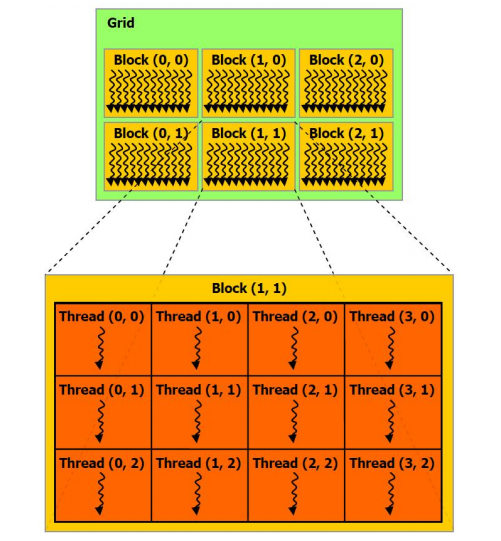
\includegraphics[scale=0.55]{images/cuda1.png}
	\caption{Organisierung von Threads in Blocks in Grids REF}
	\label{img:example_ae}
\end{figure}

\begin{enumerate}
	\item Grids, Blocks, Threads
	\item Optimierungen (?)
	\item cuda Beispiel
\end{enumerate}

\subsection{Histogramme parallel berechnen}

Ein häufig eingesetztes Muster, da es sich hervorragend  für parallele Berechnungen eignet, ist das Histogramm. Hierbei wird die Häufigkeit einer Wertmenge in Klassen eingeteilt. Histogramme finden Anwendung bei der Extraktion von Features und TODO. Eine große Menge Features kann so in k Klassen eingeteilt werden, der Anzahl oder Größe vorgegeben werden kann. Pro Feature wird die entsprechende Klasse um eins inkrementiert. Dies kann parallel durchgeführt werden da die Operation assoziativ und kommutativ ist: Es spielt keine Rolle in welcher Reihenfolge die Features abgearbeitet werden. Wenn das zu beschreibende Histogramm im global Speicher vorliegt, wird die Berechnungsgeschwindigkeit stark reduziert, da viele Threads auf die gleichen Speicheradressen des Histogramms schreibend zugreifen. Damit keine Dies wird in cuda durch die Operation \textit{atomicAdd} Um dies zu umgehen, wird pro Block in einem Grid eine lokales, privates Histogramm im shared Memory angelegt. Dadurch müssen aber noch die Werte der privaten Histogramme in das globale kumuliert werden, sobald alle Threads eines Blocks fertig sind.

\lstset{language=C}
\begin{lstlisting}
__global__
void histogram_kernel (float *buffer, long size, int *histo) {
	__shared__ int *copy[10];
	
	if (threadIdx.x < 10) {
		copy[threadIdx.x] = 0;		
	}
	__syncthreads();

	int id = threadIdx.x + blockDim.x * gridDim.x;
	int stride = blockDim.x * gridDim.x;
	
	while (i < stride) {
		int bin = buffer[i] / 10; 
		atomicAdd(&(copy[bin]), 1);
		i += stride;	
	}
	__syncthreads();
	
	if (threadIdx.x < 10) {
		atomicAdd(&(histo[threadIdx.x]), copy[threadIdx.x]);		
	}
}
\end{lstlisting} 